\chapter{idock: Protein-Ligand Docking}

Protein-ligand docking predicts the preferred conformation and binding affinity of a small ligand when it is non-covalently bound to a specific binding site of a macro protein. Up to date, there are hundreds of docking programs available \citep{493,922}. The AutoDock series is the most cited docking software in the research community. AutoDock has contributed to the discovery of several drugs, including the first clinically approved HIV integrase inhibitor \citep{1169}. Technically speaking, AutoDock is single threaded \textit{per se}. Following its initial release, several parallel implementations were developed, using either multithreading or computer cluster \citep{115,560,782}.

In 2009, AutoDock Vina \citep{595} was released. As the successor of AutoDock 4 \citep{596}, AutoDock Vina significantly improves the average accuracy of the binding mode predictions while running two orders of magnitude faster with multithreading \citep{595}. It was compared to AutoDock 4 on selecting active compounds against HIV protease, and was recommended for docking large molecules \citep{556}. Its functionality of semi-flexible protein docking by enabling flexibility of side-chain residues was evaluated on VEGFR-2 \citep{1084}. To further facilitate the usage of AutoDock Vina, auxiliary tools were subsequently developed, including a PyMOL plugin for program settings and visualization \citep{609}, and a bootable operating system for computer clusters \citep{773}. AutoDock Vina is free and open source under Apache License 2.0. So far it has been cited by over 400 publications according to Google Scholar, making it a very competitive docking program.

In 2011, inspired by AutoDock Vina, we developed idock 1.0 \citep{1153}, a multithreaded virtual screening tool for flexible ligand docking. idock inherits from AutoDock Vina the accurate scoring function and the efficient optimization algorithm, and meanwhile introduces a fruitful of innovations, such as receptor and grid map caching for large-scale virtual screening, revised numerical model for much faster approximation, capability of automatic detection and deactivation of inactive torsions, utilization of our novel thread pool to parallelize grid map creation and reuse threads, utilization of the new C++11 feature of rvalue references to avoid frequent memory reallocation, and accelerated parsers for both receptor and ligand. When benchmarked on docking 10,928 drug-like ligands against HIV reverse transcriptase, idock 1.0 achieved a speedup of 3.3 in terms of CPU time and a speedup of 7.5 in terms of elapsed time on average compared to AutoDock Vina.

Despite the amazing speedup, idock 1.0 still required about 10 hours on average to dock 10,928 drug-like ligands, not to mention massive docking of millions of ligands. Faster algorithms and implementations are highly desired. Following the release of idock 1.0 in July 2011, we then released idock 1.1 in December 2011, idock 1.2 in February 2012, idock 1.3 in March 2012, idock 1.4 in April 2012, idock 1.5 in June 2012, and idock 1.6 in August 2012, further improving docking speed and accuracy, inventing new functionalities, and fixing bugs. Refer to table \ref{idock:Releases} for change log in detail.

\begin{table}
\centering
\begin{tabular*}
{\linewidth}
{@{\extracolsep{\fill}}ccp{0.7\textwidth}}
\toprule
Version & Date & Change Log \\
\midrule
1.0 & Jul 2011 & Initial release at CodePlex. Revised numerical approximation model. Automatic detection and deactivation of inactive torsions. Flattened the tree-like recursive data structure of ligand as used in AutoDock Vina into simple linear array structure to ensure a high data cache hit rate and easy coding.\\
1.1 & Dec 2011 & Project migrated from CodePlex to GitHub. Tested Solaris 11, clang 3.0, and Intel C++ Compiler v11. Added precompiled executables for both 32-bit and 64-bit Linux and Windows. Added thread-safe progress bar. Output predicted free energy of the top 5 conformations. Improved the evaluation of intra-molecular free energy.\\
1.2 & Feb 2012 & Added program option csv for dumping docking summary sorted in the ascending of predicted free energy. Profiled by the Valgrind tool suite to ensure zero memory leak. Revised the precision of coordinates and free energy to be 3 digits. Parallelized the precalculation of scoring function. Added support for Mac OS X 10.7.2 and FreeBSD 9.0.\\
1.3 & Mar 2012 & Implemented a lightweight quaternion class. Added bash scripts for running AutoDock Vina for docking ZINC clean drug-like ligands. Output predicted total free energy, inter-ligand free energy, intra-ligand free energy, and per-atom free energy to docked PDBQT files. Added a new example 1V9U.\\
1.4 & Apr 2012 & Fixed a segmentation fault bug when the number of heavy atoms exceeds 100. Added two new examples 2IQH and 1HCL. Skipped already docked ligands. Prevented dead loop by limiting the number of initial conformation trials.\\
1.5 & Jun 2012 & Added a new example 2ZNL. Supported a new chemical element strontium (Sr). Supported file error detection in output folder. Supported reading and writing ligands in gzip and/or bzip2 format. Output the number of hydrogen bonds for each conformation.\\
1.6 & Aug 2012 & Added a new example 2VQZ. Output putative inter-molecular hydrogen bonds for each predicted conformation. Precompiled idock for Windows using Visual Studio 2012. Supported CentOS 6.3. Upgraded boost from 1.50.0 to 1.51.0.\\
\bottomrule
\end{tabular*}
\caption{idock releases and change log.}
\label{idock:Releases}
\end{table}

\section{Methods and Contributions}

Figure \ref{idock:Flowchart} shows the overall flowchart of idock. During initialization, idock precalculates the scoring function for all possible combinations of atom type pairs and interatomic distances. It parses the receptor and determines the atom types with the aid of residue sequence, and creates a thread pool to hold reusable threads. Then it enters a loop and fetches a ligand from a user-specified input folder to perform docking. It parses the ligand and determines the atom types with the aid of branch information, and meanwhile automatically detects and deactivates inactive torsions. It builds grid maps of granularity 0.15625 \AA\ by default on the fly by multithreading, and distributes multiple independent Monte Carlo tasks to the thread pool for concurrent execution. Then it merges the conformations from separate threads and clusters them with RMSD 2.0 \AA, and dumps them to the user-specified output folder and displays the predicted free energy on screen. It proceeds with the next ligand automatically until all are docked. Finally it destroys the thread pool and releases memory resources.

\begin{figure}
\centering
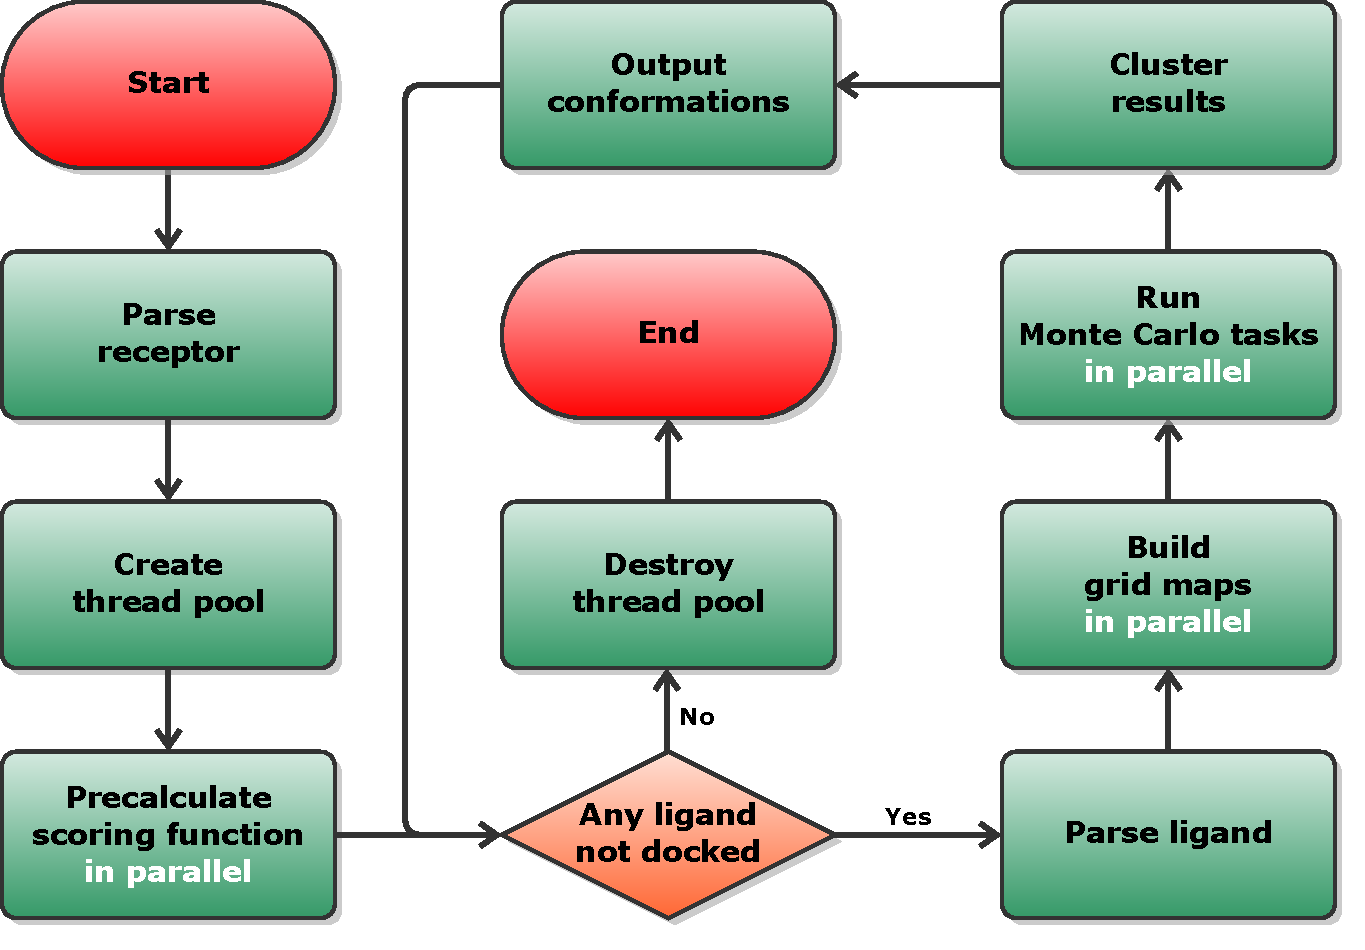
\includegraphics[width=\linewidth]{idock/Flowchart.pdf}
\caption{Flowchart of idock.}
\label{idock:Flowchart}
\end{figure}

\subsection{Scoring Function}

Both idock and Vina share exactly the same scoring function, which is made up of a conformation-dependent part and a conformation-independent part. The conformation-dependent part is a weighted sum of five terms over all the pairs of atom $i$ and atom $j$ that can move relative to each other. It is calculated from equations \eqref{eqn:e} and \eqref{eqn:eij} where $t_i$ and $t_j$ are the atom types of $i$ and $j$ respectively, and $r_{ij}$ is their interatomic distance. The five terms are calculated from equations \eqref{eqn:Gauss1} to \eqref{eqn:HBonding} where $d_{ij}$ is the surface distance calculated from equation \eqref{eqn:dij} where $R_{t_i}$ and $R_{t_j}$ are the Van der Waals radii of $t_i$ and $t_j$ respectively (Figure \ref{idock:Distance}). All the units are in \AA. The weighting coefficients and the cut off at $r_{ij}$ = 8 \AA\ of the five terms are borrowed from Vina. The optimization algorithm attempts to find the global minimum of $e$ and other low-scoring conformations, which it then ranks.
\begin{equation}
\label{eqn:e}
e = \sum_{i < j} e_{ij}
\end{equation}
\begin{eqnarray}
\label{eqn:eij}
e_{ij} &=& (-0.035579) * Gauss_1(t_i, t_j, r_{ij}) \nonumber \\
       &+& (-0.005156) * Gauss_2(t_i, t_j, r_{ij}) \nonumber \\
       &+& (+0.840245) * Repulsion(t_i, t_j, r_{ij}) \nonumber \\
       &+& (-0.035069) * Hydrophobic(t_i, t_j, r_{ij}) \nonumber \\
       &+& (-0.587439) * HBonding(t_i, t_j, r_{ij})
\end{eqnarray}
\begin{equation}
\label{eqn:Gauss1}
Gauss_1(t_i, t_j, r_{ij}) = e^{-(d_{ij} / 0.5)^2}
\end{equation}
\begin{equation}
\label{eqn:Gauss2}
Gauss_2(t_i, t_j, r_{ij}) = e^{-((d_{ij} - 3) / 2)^2}
\end{equation}
\begin{equation}
\label{eqn:Repulsion}
Repulsion(t_i, t_j, r_{ij}) =
\begin{cases}
d_{ij}^2 & \text{if } d_{ij} < 0\\
0 &\text{if } d_{ij} \geq 0
\end{cases}
\end{equation}
\begin{equation}
\label{eqn:Hydrophobic}
Hydrophobic(t_i, t_j, r_{ij}) =
\begin{cases}
1 & \text{if } d_{ij} \leq 0.5\\
1.5 - d_{ij} & \text{if } 0.5 < d_{ij} < 1.5\\
0 & \text{if } d_{ij} \geq 1.5\\
\end{cases}
\end{equation}
\begin{equation}
\label{eqn:HBonding}
HBonding(t_i, t_j, r_{ij}) =
\begin{cases}
1 & \text{if } d_{ij} \leq -0.7\\
d_{ij} / (-0.7) & \text{if } -0.7 < d_{ij} < 0\\
0 & \text{if } d_{ij} \geq 0\\
\end{cases}
\end{equation}
\begin{equation}
\label{eqn:dij}
d_{ij} = r_{ij} - (R_{t_i} + R_{t_j})
\end{equation}

\begin{figure}
\centering
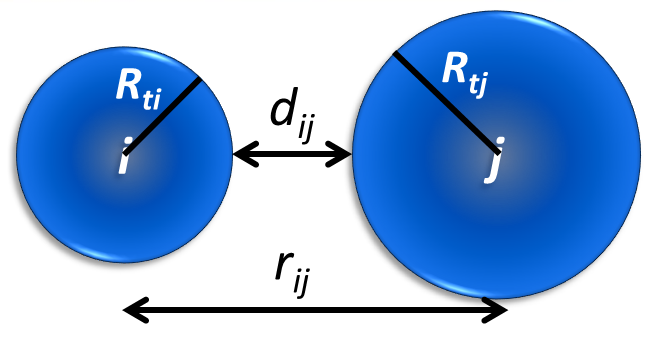
\includegraphics[width=\linewidth]{idock/Distance.png}
\caption{Relationship between surface distance $d_{ij}$ and interatomic distance $r_{ij}$.}
\label{idock:Distance}
\end{figure}

The conformation-dependent part can be seen as the sum of intermolecular and intramolecular contributions. Hence equation \eqref{eqn:e} can be rewritten into equation \eqref{eqn:inter-intra} where $e_{inter}$ is the summation over all the heavy atoms between receptor and ligand, and $e_{intra}$ is the summation over all the 1-4 ligand heavy atoms that are separated by three consecutive covalent bonds and can move relative to each other.
\begin{equation}
\label{eqn:inter-intra}
e = e_{inter} + e_{intra}
\end{equation}
The conformation-independent part penalizes $e_{inter}$ for ligand flexibility. The predicted free energy of the $k$th conformation for output, denoted as $e'_k$, is calculated from equation \eqref{eqn:FlexibilityPenalty} where $k$ is the subscript for conformation, $e_k$ is the conformation-dependent score of the $k$th conformation calculated from equation \eqref{eqn:e}, $e_{intra,1}$ is the $e_{intra}$ of the first, i.e. lowest-scoring conformation, $N_{ActTors}$ is the number of active torsions and $N_{InactTors}$ is the number of inactive torsions of the ligand. Note that $e_{intra,1}$, rather than $e_{intra,k}$, acts as subtrahend in order to preserve the ranking.
\begin{equation}
\label{eqn:FlexibilityPenalty}
e'_k = \frac{e_k - e_{intra,1}}{1 + 0.05846 * (N_{ActTors} + 0.5 * N_{InactTors})}
\end{equation}
The value of $e_{ij}$ is basically a function of three variables, namely $t_i$, $t_j$, and $r_{ij}$. These three variables have both a known lower bound and a known upper bound, so it is possible to precalculate the scoring function. Since there are 17 atom types implemented in idock, the pair of $t_i$ and $t_j$ can have 153 (=17*18/2) different combinations. Since $r_{ij}$ is cut off at 8 \AA, idock uniformly samples 16,384 points in range [0, 8] to turn the continuous domain into a concrete domain, resulting in an average absolute error of merely 0.002 kcal/mol. During program initialization, idock precalculates $e_{ij}$ from equation \eqref{eqn:eij} for 153*16384 possible combinations of $t_i$, $t_j$, and $r_{ij}$. During optimization, idock approximates the true value of $e_{ij}$ by direct assignment rather than linear interpolation for faster evaluation of $e_{ij}$ at the cost of a little bit longer precalculation time and a bit more memory storage.

\subsection{Grid Maps}

In order to fast evaluate $e_{inter}$, grid maps are often built. A grid map of atom type \textit{t} is constructed by placing virtual probe atoms of atom type \textit{t} along the X, Y, Z dimensions of the search box at a certain granularity (Figure \ref{idock:GridMap}). The $e_{inter}$ value of these probe atoms are precalculated, so the $e_{inter}$ value of a ligand heavy atom can be approximated in some way. In Vina, the grid map granularity is hard coded to be 0.375 \AA, and the approximation is done by linear interpolation of the 8 corner probe atoms of the residing subbox. This kind of interpolation involves reading of 8 $e_{inter}$ values, computation of 3 $\alpha$ values, 12 floating-point subtractions, 24 floating-point multiplications, and 7 floating-point additions, which turned out to be a performance bottleneck when we profiled Vina. In contrast, idock exposes grid map granularity as an optional program argument with a tuned default value of 0.15625 \AA. Likewise, due to a higher density of probe atoms, idock substitutes direct assignment for linear interpolation for much faster evaluation of $e_{inter}$ at the cost of longer precalculation time and larger memory storage. Therefore, the creation of grid maps is carried out on the fly only when necessary and abstracted into parallel tasks, which are then distributed to the thread pool for concurrent execution.

\begin{figure}
\centering
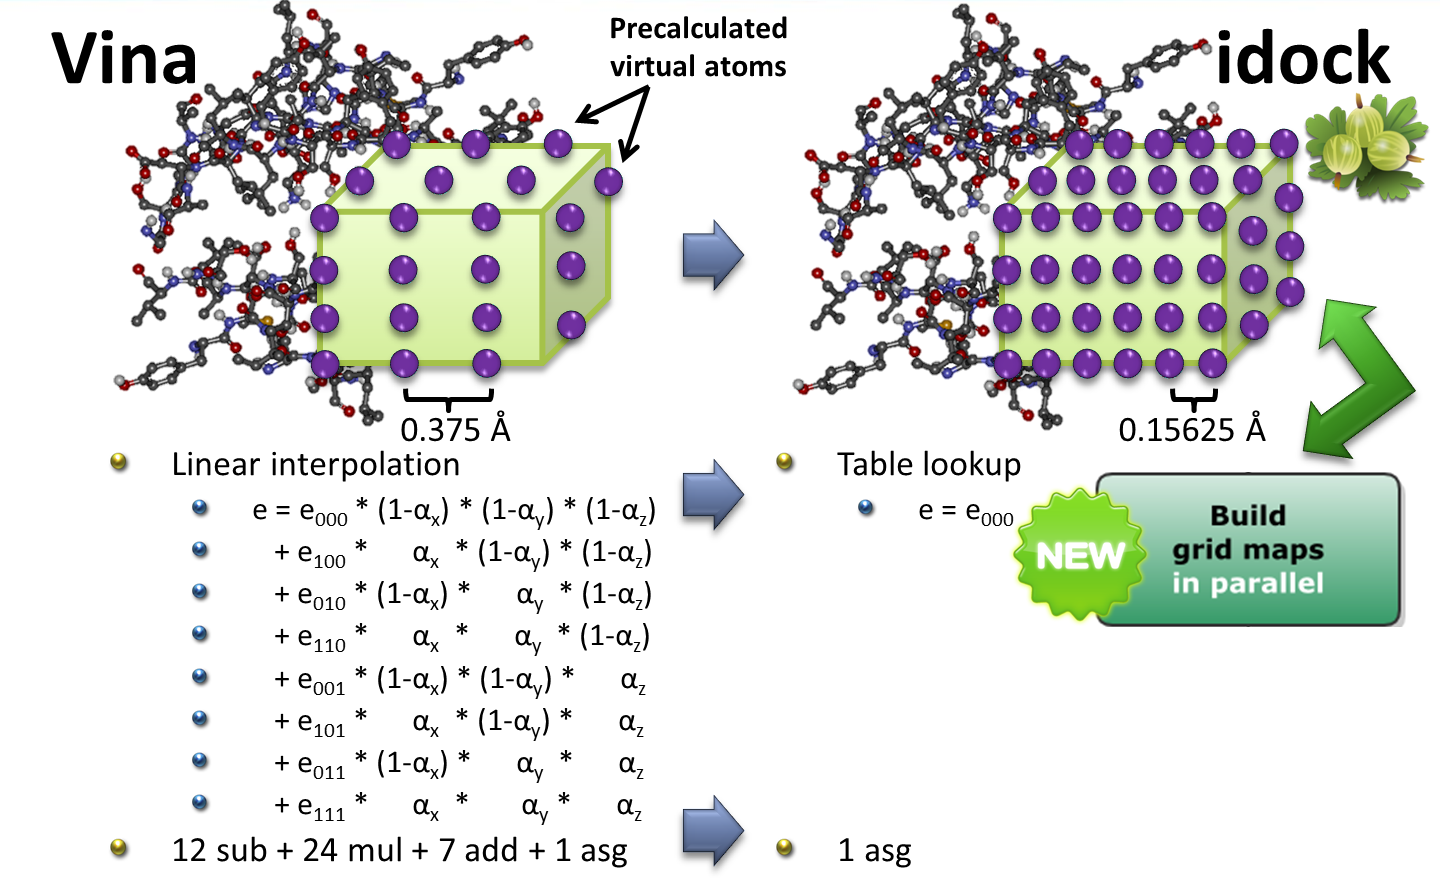
\includegraphics[width=0.5\linewidth]{idock/GridMap.png}
\caption{Grid map for fast evaluation of $e_{inter}$. Probe atoms are shown in purple.}
\label{idock:GridMap}
\end{figure}

\subsection{Optimization Algorithm}

Both idock and Vina use Monte Carlo algorithm for global optimization and Broyden-Fletcher-Goldfarb-Shanno (BFGS) \cite{786} Quasi-Newton method for local optimization. A succession of steps consisting of a mutation and a BFGS local optimization are taken, with each step being accepted according to the Metropolis criterion (Figure \ref{idock:MonteCarlo}, modified from \cite{493}). These steps are repeated over \textit{N} iterations, where \textit{N} correlates to the complexity of the ligand regarding number of heavy atoms and number of torsions. BFGS approximates the inverse Hessian matrix of the scoring function. It uses not only the value of the scoring function but also its gradient, which are the derivatives of the scoring function with respect to the position and orientation of the ligand, and the torsions for the active rotatable bonds in the ligand. A BFGS iteration derives a descent direction from the approximate inverse Hessian matrix, derives a step length along the descent direction by line search, and updates the approximation of inverse Hessian matrix. Both programs achieve multithreading by concurrently running multiple independent Monte Carlo tasks starting from random initial conformations.

\begin{figure}
\centering
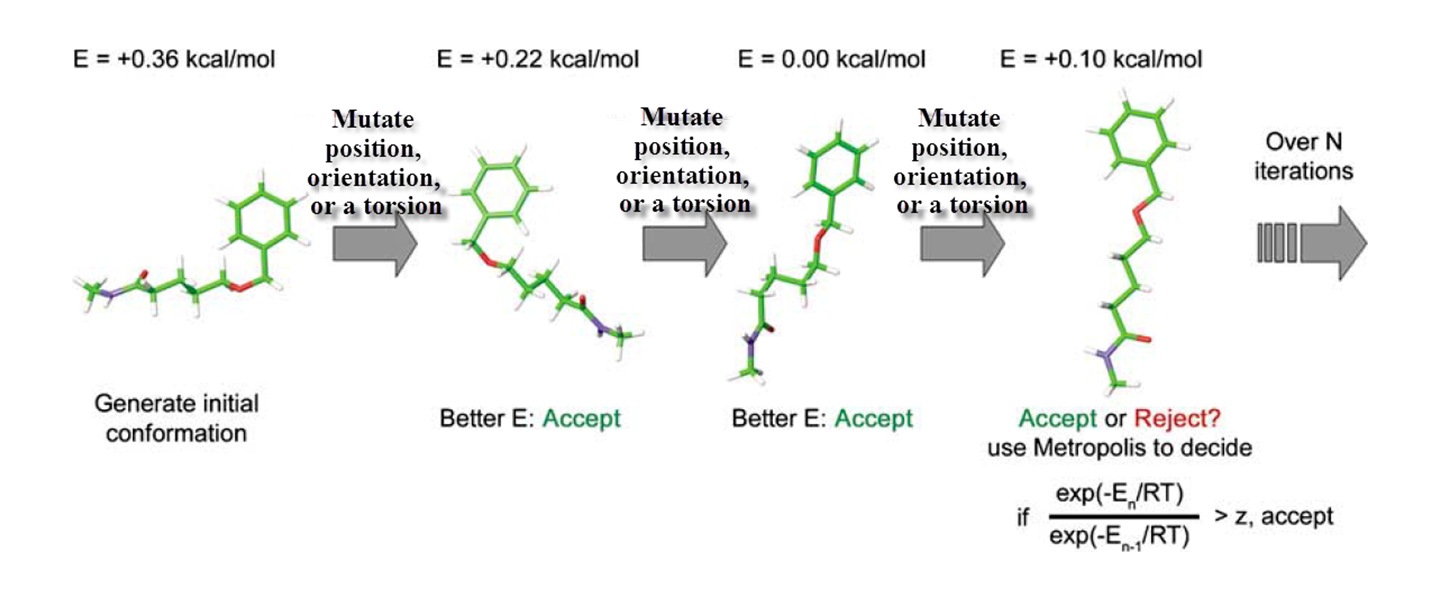
\includegraphics[width=\linewidth]{idock/MonteCarlo.png}
\caption{Monte Carlo algorithm for docking. Figure modified from \cite{493}.}
\label{idock:MonteCarlo}
\end{figure}

Though both programs share similar optimization algorithms, their implementations differ. Compared with Vina, the Monte Carlo iterations in idock are far fewer and the BFGS iterations are more. On one hand, the fewer number of Monte Carlo iterations is compensated by a larger number of parallel Monte Carlo tasks, which is 64 by default in idock compared to 8 in Vina, guaranteeing better conformational diversity and higher CPU utilization on multi-core computers. On the other hand, the stopping criterion of BFGS local optimization does not depend on an estimated number of iterations, which is the case in Vina, but depends on the outcome of line search. The BFGS local optimization stops if and only if no appropriate step length can be obtained by line search, thus increasing the probability of finding optimal local minimums.

\subsection{Native Support of Virtual Screening}

Vina is optimized for single-ligand docking rather than virtual screening. When it comes to docking a large pool of ligands, Vina has to be invoked multiple times, repeatly parsing the same receptor and creating the same grid maps, and thus degrading performance.

idock supports virtual screening in a native manner. It reuses receptor and grid maps. Given a very large amount of ligands to dock, idock indirectly supports 2-phase virtual screening via two consecutive runs. In the first run, idock performs coarse but fast virtual screening without writing any conformations to file, aiming to quickly shortlist a few candidate compounds. In the second run, idock performs fine but slow virtual screening with a significantly larger number of Monte Carlo tasks per ligand, writing as many conformations to file as possible and aiming to refine the predicted free energy as well as predicted conformation of candidate compounds. Such a 2-phase docking methodology can remarkably reduce overall execution time while avoiding the risk of filtering out potentially promising compounds, controlling the false negative rate at an acceptable level.

\subsection{Novel Thread Pool}

idock implements our novel thread pool in order to reuse threads and maintain a high CPU utilization throughout the entire screening procedure. The thread pool parallelizes the precalculation of scoring function, the creation of grid maps, and the execution of Monte Carlo tasks.

\subsection{Detection of Inactive Torsions}

idock automatically detects and deactivates inactive torsions, which are presented and activated in the input file in pdbqt format but have no impact on the overall scoring, such as \textemdash{OH} and \textemdash{NH$_2$}, because they only rotate the hydrogens. Figure \ref{idock:InactiveTorsions} shows an example ligand which contains 4 active torsions defined by the python script \textit{prepare\_ligand4.py} provided by AutoDock Tools \cite{785,596}. Two of them, highlighted in yellow, only rotate hydrogens and thus have no contributions to the scoring. They are re-classified as inactive torsions and deactivated while being parsed in idock. This kind of automatic detection and deactivation of inactive torsions reduces the dimension of variables to optimize in the local optimization step, leading to easier finding of local minimums.

\begin{figure}
\centering
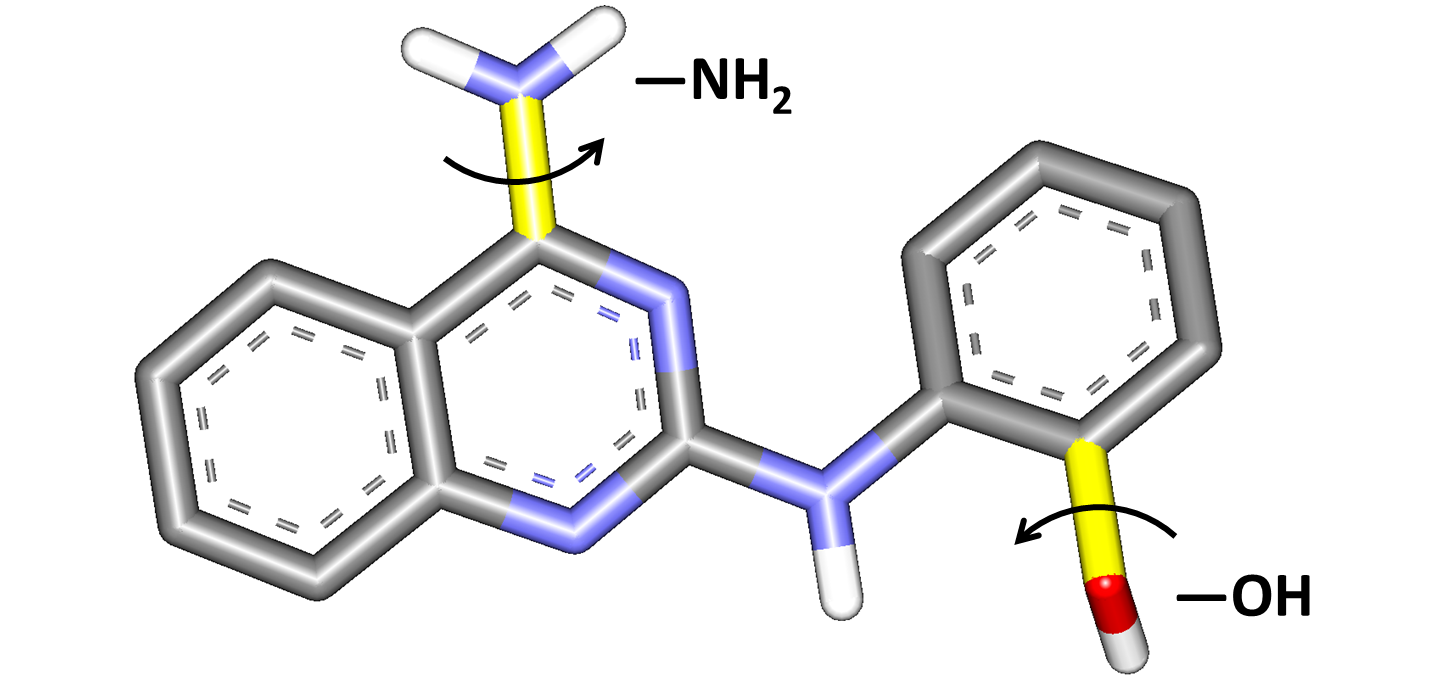
\includegraphics[width=0.5\linewidth]{idock/InactiveTorsions.png}
\caption{Example of inactive torsions highlighted in yellow. Nonpolar hydrogens are not shown for clarity.}
\label{idock:InactiveTorsions}
\end{figure}

\subsection{Automatic Recovery}

idock enables automatic recovery. In case the process gets killed accidentally and restarted some time later, it not only resumes docking from the previous stopping point, skipping ligands that were already docked in a previous run, but also detects and reports possible file content errors, ensuring all the output ligands are well written.

\subsection{Gzip/Bzip2 Compression}

idock supports reading and writing compressed ligand files with in gzip/bzip2 format, resulting in a file footprint as low as just one eighth of the raw size. This new functionality turns out to be extremely handy given an enormous amount of ligands to dock.

\subsection{Verbose Output}

idock evaluates and outputs verbose information to docked PDBQT files (Figure \ref{idock:OutputPDBQT}), including total free energy, total inter-ligand free energy, total intra-ligand free energy, hydrogen bonds, and per-atom inter-ligand free energy, facilitating interaction hotspot determination and indirectly helping \textit{in silico} synthesis of potent ligands, improving potency by altering certain chemical moieties of known ⁄ endogenous ligands while retaining those critical for binding.

\begin{figure}
\centering
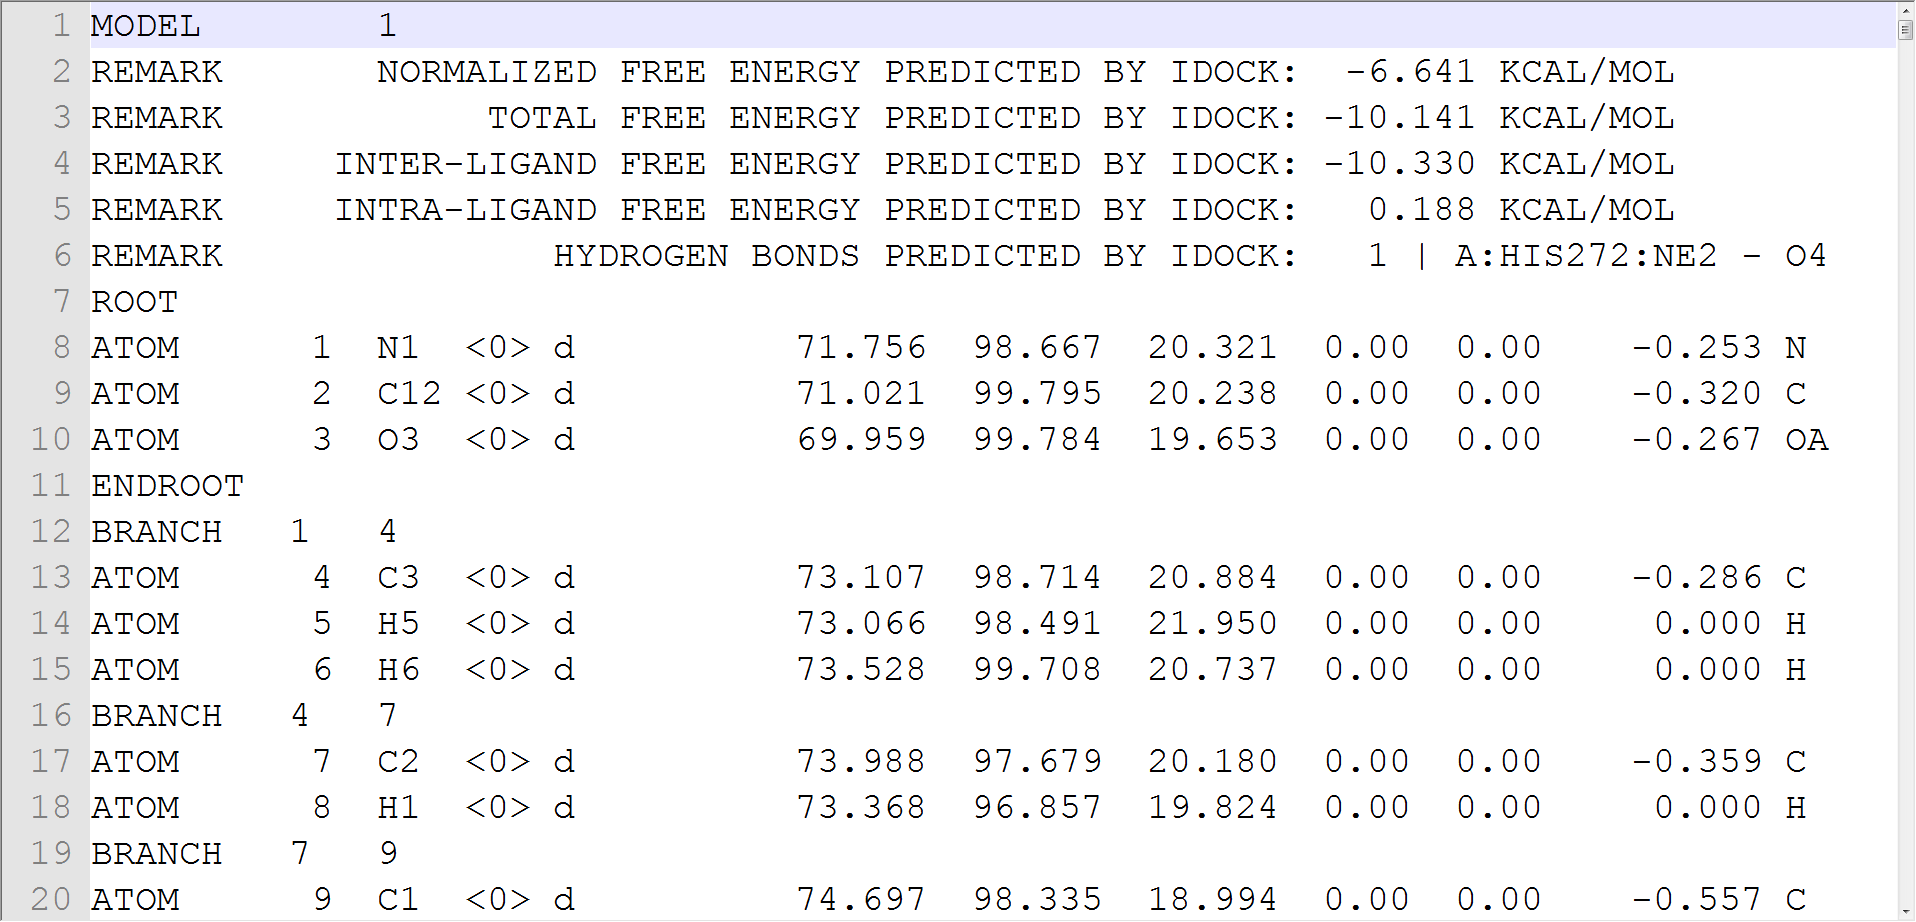
\includegraphics[width=\textwidth]{idock/OutputPDBQT.png}
\caption{Verbose output of idock in PDBQT format.}
\label{idock:OutputPDBQT}
\end{figure}

idock writes docking summary, sorted in the ascending order of predicted free energy of docked ligands, in CSV (Comma-Separated Vector) format for subsequent analysis easily (Figure \ref{idock:OutputCSV}).

\begin{figure}
\centering
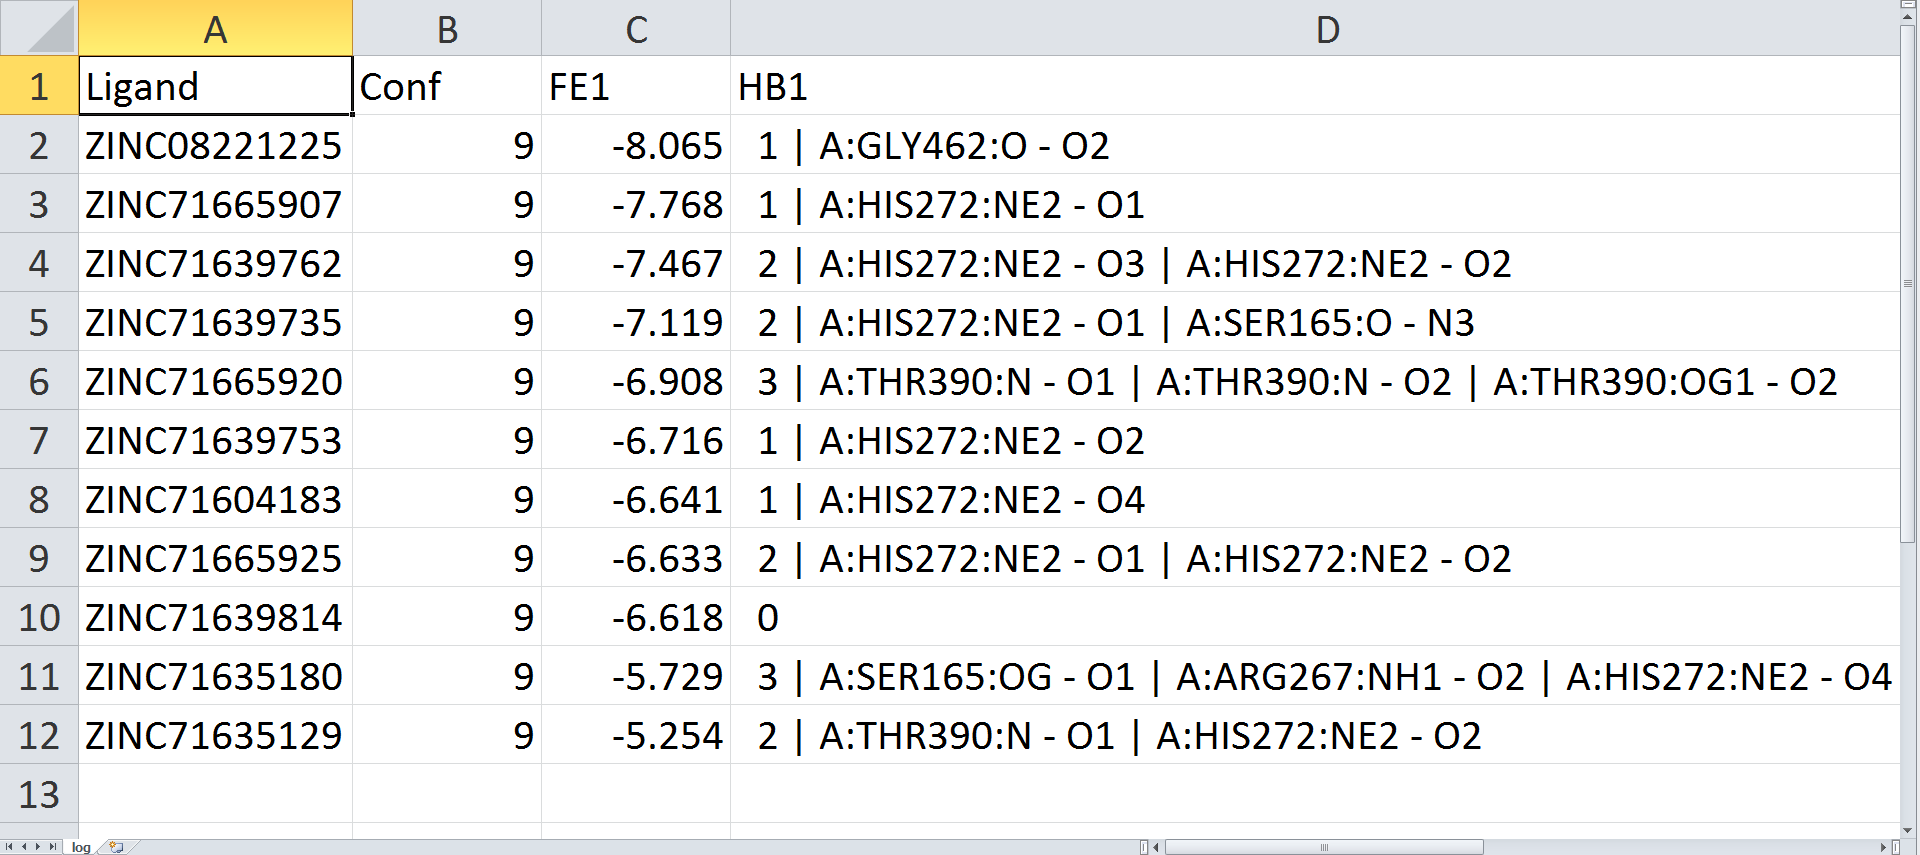
\includegraphics[width=\textwidth]{idock/OutputCSV.png}
\caption{Summary output of idock in CSV format.}
\label{idock:OutputCSV}
\end{figure}

\subsection{Chemical Elements}

It supports as many as 29 chemical elements including rare ones like As (arsenic) and Sr (strontium), covering the majority of ligand atom types.
%Periodic Table of Elements

\subsection{Full Reproducibility}

We emphasize full reproducibility, which has the potential to serve as a minimum standard for judging scientific claims when full independent replication of a study is not possible \citep{965}. idock supports Linux, Windows, Mac OS X, FreeBSD and Solaris, making it instantly ready on the 5 mainstream operating systems. Accompanying with idock are 13 ready-to-use docking examples, a doxygen file for generating API documentations, and 2 graphical tutorials.

\subsection{Miscellaneous Enhancements}

idock implements our own lightweight thread-safe progress bar, reporting progress every 10\% Monte Carlo tasks per ligand. idock better supports rvalue references and move semantics in C++11 to boost performance. idock flattens the tree-like recursive data structure of ligand as used in AutoDock Vina into simple linear array structure to ensure a high data cache hit rate and easy coding. idock accelerates the assignment of atom types by making use of residue information for receptor and branch information for ligand.

\section{Benchmarks and Results}

idock x86\_64 v1.5 and AutoDock Vina x86 v1.1.2 were evaluated on desktop computers with Intel Core i5-2400 CPU @ 3.10GHz and 4GB DDR3 RAM under Mac OS X 10.7.4 Build 11E53. Arguments to both programs were left as default. By default, both programs output 9 predicted conformations per ligand. The benchmarks include comparison of their redocking performance in terms of predicted conformations, and comparison of their virtual screening performance in terms of execution time, memory usage, predicted free energy, and predicted conformations.

\subsection{Benchmark of Redocking}

Redocking refers to randomizing the crystal ligand conformation in a protein-ligand complex and trying to dock the randomized conformation back to its crystal conformation as close as possible. For the redocking benchmark, we used two databases, PDBbind v2011 \citep{529,530} and CSAR NRC HiQ Set 24Sept2010 \citep{857,960}. The refined set of PDBbind v2011 and the two sets of CSAR NRC HiQ Set 24Sept2010 comprise 2,455 and 343 protein-ligand complexes respectively, with experimentally determined binding affinity data (Kd or Ki).

Table \ref{idock:SuccessRate} shows the success rates of idock and AutoDock Vina under various conditions regarding the RMSD values between the crystal and docked conformations. Given a redocking case, RMSD1 refers to the RMSD value between the crystal conformation and the first docked conformation, i.e. the one with the highest predicted binding affinity, while RMSDm refers to the RMSD value between the crystal conformation and the closest docked conformation, i.e. the one with the minimum RMSD value. The condition RMSD1 = RMSDm tests for how many percent the docked conformation with the highest predicted binding affinity actually turns out to be the closest one among the 9 predicted conformations. It can be seen that the success rates of idock are comparable to, albeit slightly lower than, AutoDock Vina, and the success rates on CSAR NRC HiQ Set 24Sept2010 are consistently higher than PDBbind v2011, probably because the scoring function performs well on carefully refined structures. Using a RMSD value of 2.0 \AA, a publicly accepted positive control for correct bound structure prediction, both programs manage to predict a conformation close enough to the crystal conformation as the first conformation for over half of the cases on both databases.

\begin{table}
\centering
\begin{tabular*}
{\linewidth}
{@{\extracolsep{\fill}}crrrr}
\toprule
& \multicolumn{2}{c}{PDBbind v2011} & \multicolumn{2}{c}{CSAR NRC HiQ}\\
Condition & idock & Vina & idock & Vina\\
\midrule
RMSD1 = RMSDm   & 47\% & 54\% & 57\% & 71\%\\
RMSD2 = RMSDm   & 16\% & 14\% & 17\% & 13\%\\
RMSD3 = RMSDm   &  8\% &  8\% &  7\% &  4\%\\
RMSD4 = RMSDm   &  6\% &  5\% &  5\% &  3\%\\
RMSD5 = RMSDm   &  5\% &  5\% &  4\% &  1\%\\
RMSD6 = RMSDm   &  5\% &  4\% &  3\% &  3\%\\
RMSD7 = RMSDm   &  5\% &  4\% &  1\% &  2\%\\
RMSD8 = RMSDm   &  4\% &  3\% &  3\% &  2\%\\
RMSD9 = RMSDm   &  4\% &  3\% &  3\% &  2\%\\
RMSD1 < 0.5 \AA & 11\% & 12\% & 21\% & 21\%\\
RMSD1 < 1.0 \AA & 29\% & 31\% & 40\% & 47\%\\
RMSD1 < 1.5 \AA & 45\% & 47\% & 61\% & 67\%\\
RMSD1 < 2.0 \AA & 53\% & 56\% & 68\% & 73\%\\
RMSDm < 0.5 \AA & 14\% & 15\% & 24\% & 26\%\\
RMSDm < 1.0 \AA & 39\% & 40\% & 54\% & 55\%\\
RMSDm < 1.5 \AA & 64\% & 65\% & 78\% & 84\%\\
RMSDm < 2.0 \AA & 74\% & 78\% & 86\% & 92\%\\
\bottomrule
\end{tabular*}
\caption{Success rates of idock and AutoDock Vina under various conditions on PDBbind v2011 and CSAR NRC HiQ Set 24Sept2010.}
\label{idock:SuccessRate}
\end{table}

Figure \ref{idock:Redocking} visualizes the redocking results of four cases.

\begin{figure*}
\centering
\subfloat[PDB ID 1B8N. Vina RMSD1 = 0.139 \AA. idock RMSD1 = 0.127 \AA.]
{
  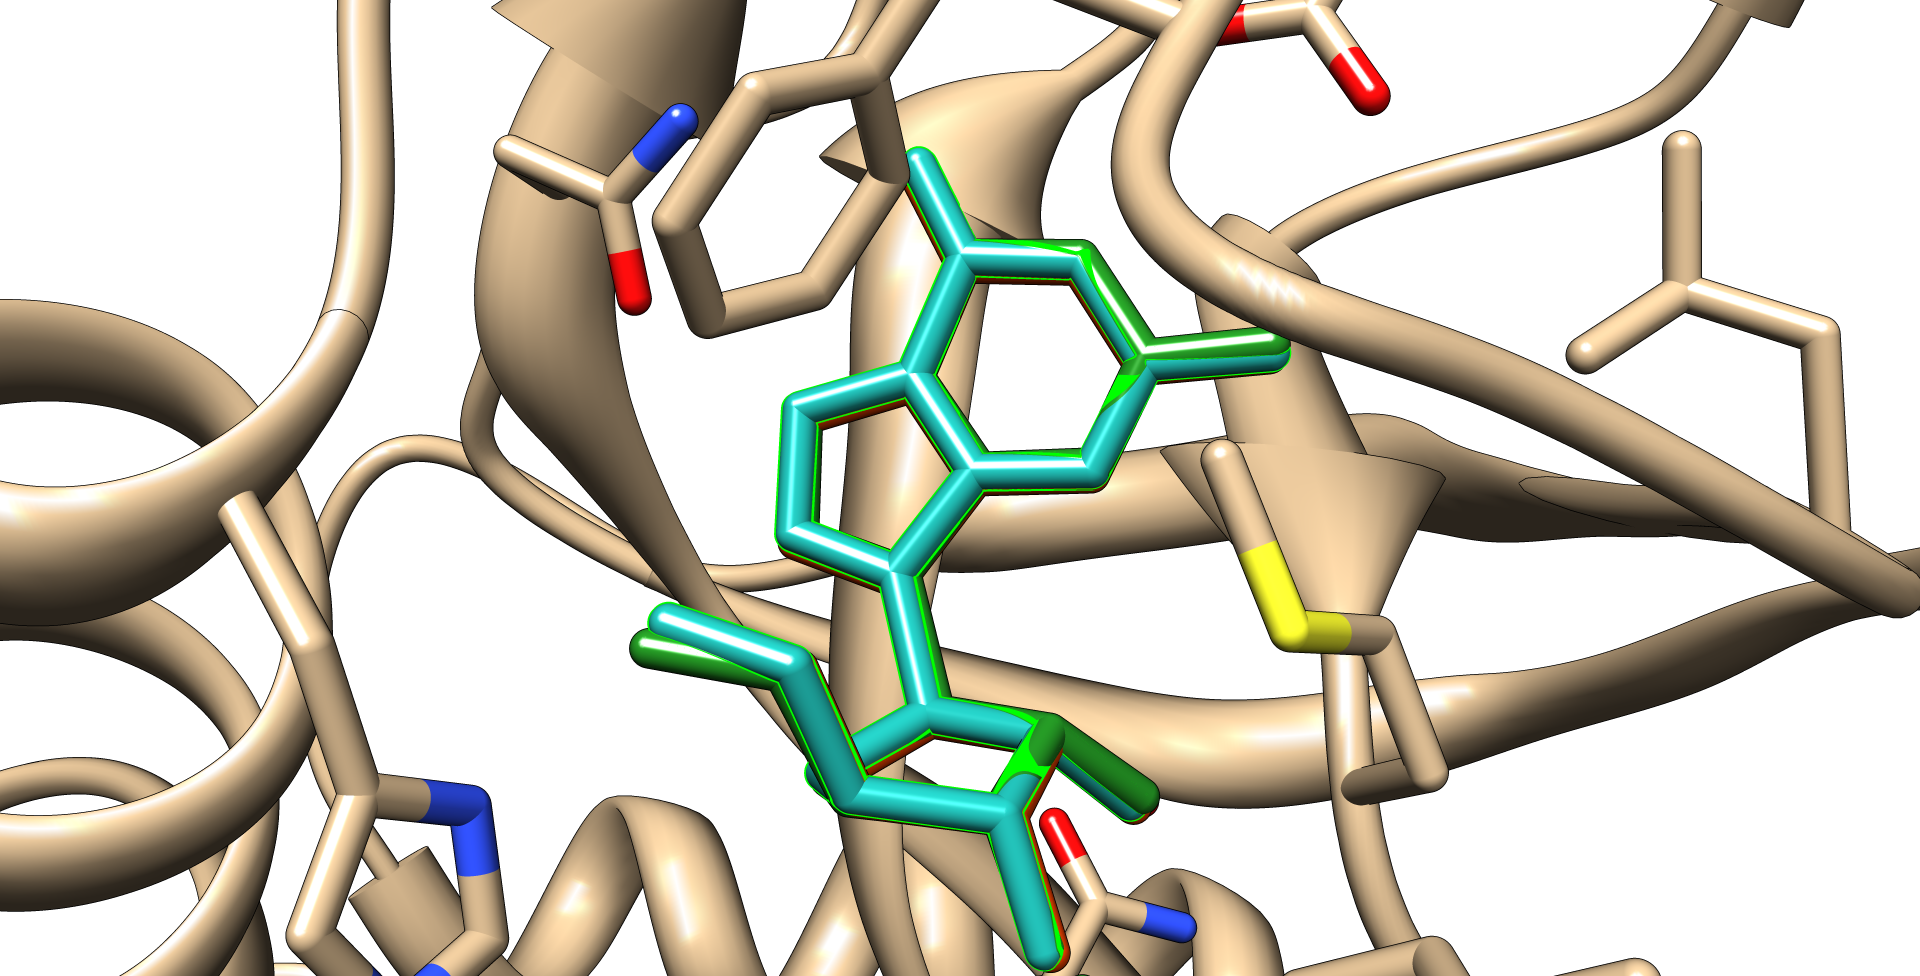
\includegraphics[width=0.485\linewidth]{idock/Redocking1B8N.png}
}
\subfloat[PDB ID 4TMN. Vina RMSD1 = 8.401 \AA. idock RMSD1 = 9.909 \AA.]
{
  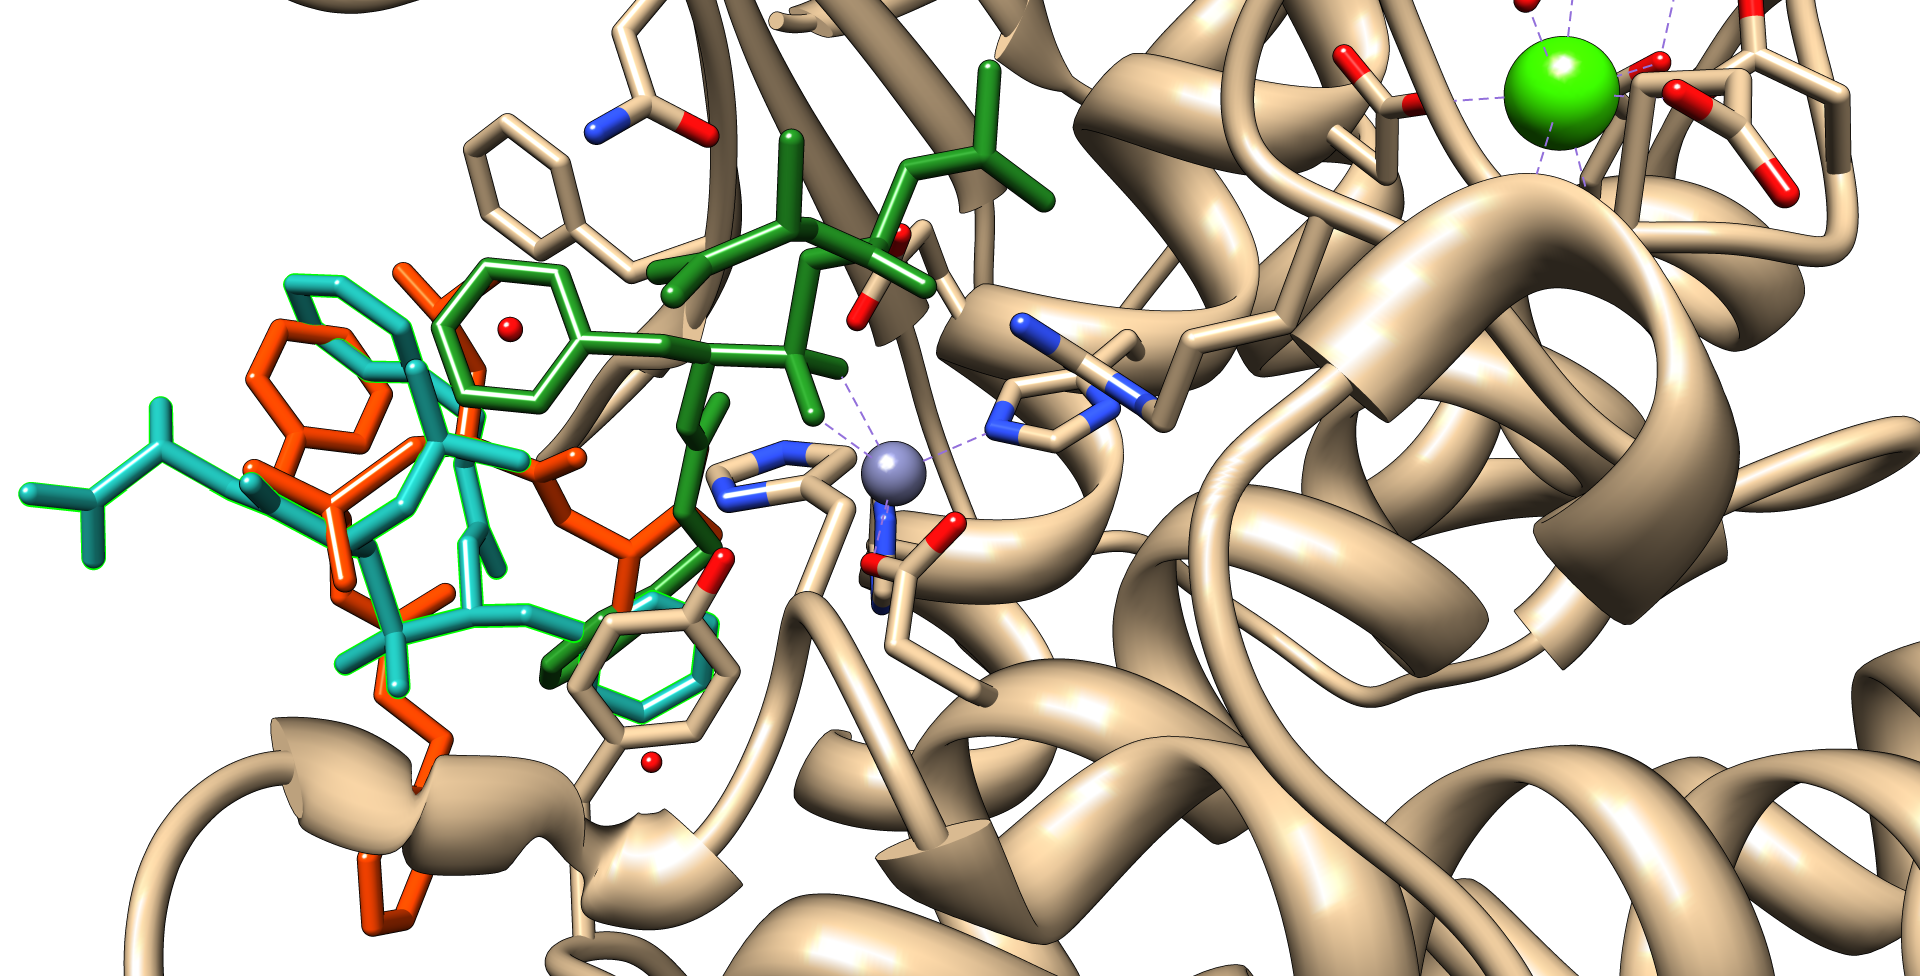
\includegraphics[width=0.485\linewidth]{idock/Redocking4TMN.png}
}
\\
\subfloat[PDB ID 1PKX. Vina RMSD1 = 7.059 \AA. idock RMSD1 = 0.214 \AA.]
{
  \includegraphics[width=0.485\linewidth]{idock/Redocking1PKX.png}
}
\subfloat[PDB ID 3HV8. Vina RMSD1 = 0.290 \AA. idock RMSD1 = 10.232 \AA.]
{
  \includegraphics[width=0.485\linewidth]{idock/Redocking3HV8.png}
}
\caption{Redocking results of four cases.}
\label{idock:Redocking}
\end{figure*}

Figure \ref{idock:FECorrelation} shows the free energy correlation of idock and AutoDock Vina. On the CSAR NRC HiQ Set 24Sept2010 database, the Pearson correlations between experimental binding affinity and free energy predicted by AutoDock Vina, between experimental binding affinity and free energy predicted by idock, and between free energy predicted by AutoDock Vina and idock are -0.5998758, -0.5774972, and 0.9824049, respectively. The experimental binding affinity is positive while the predicted free energy is negative, hence the negative sign for the former two correlations. It can be seen that both programs fail to predict reliable free energy, a very common obstacle in the entire research community. As expected, the correlation between free energy predicted by both programs is very close to 1 because of their identical scoring function.

\begin{figure*}
\centering
\subfloat[PDBbind v2011]
{
  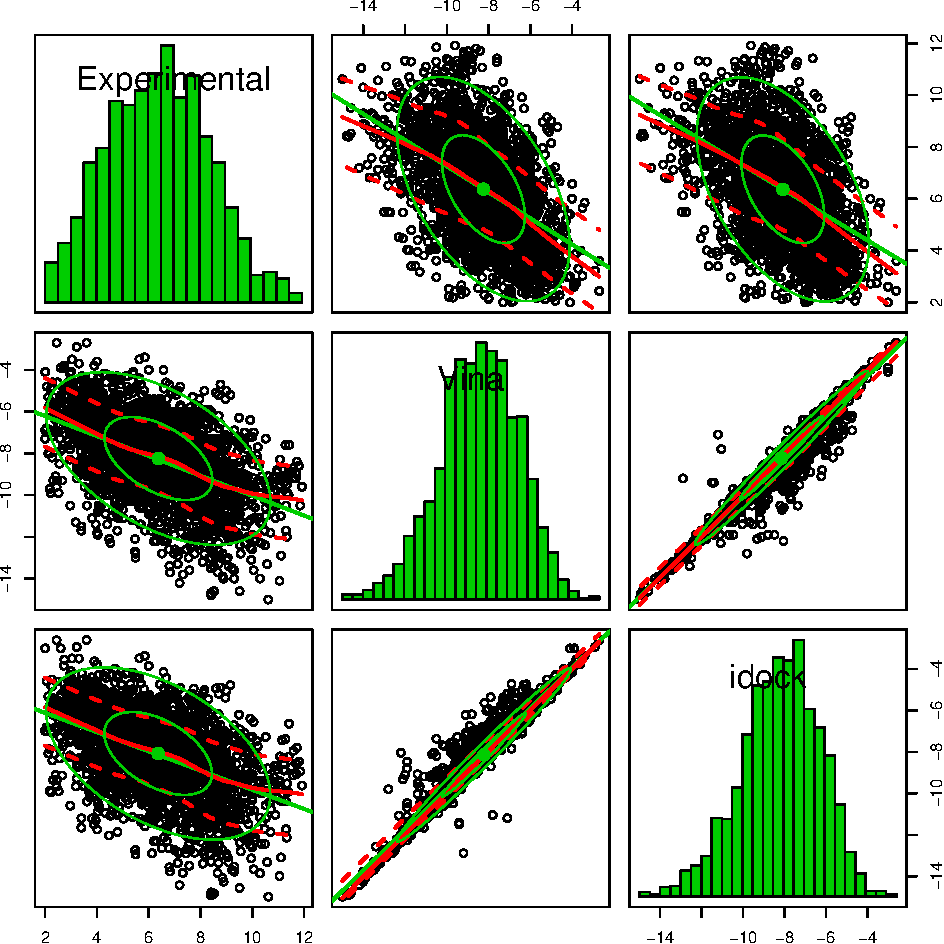
\includegraphics[width=0.485\linewidth]{idock/PDBbindFECorrelation.pdf}
}
\subfloat[CSAR NRC HiQ Set 24Sept2010]
{
  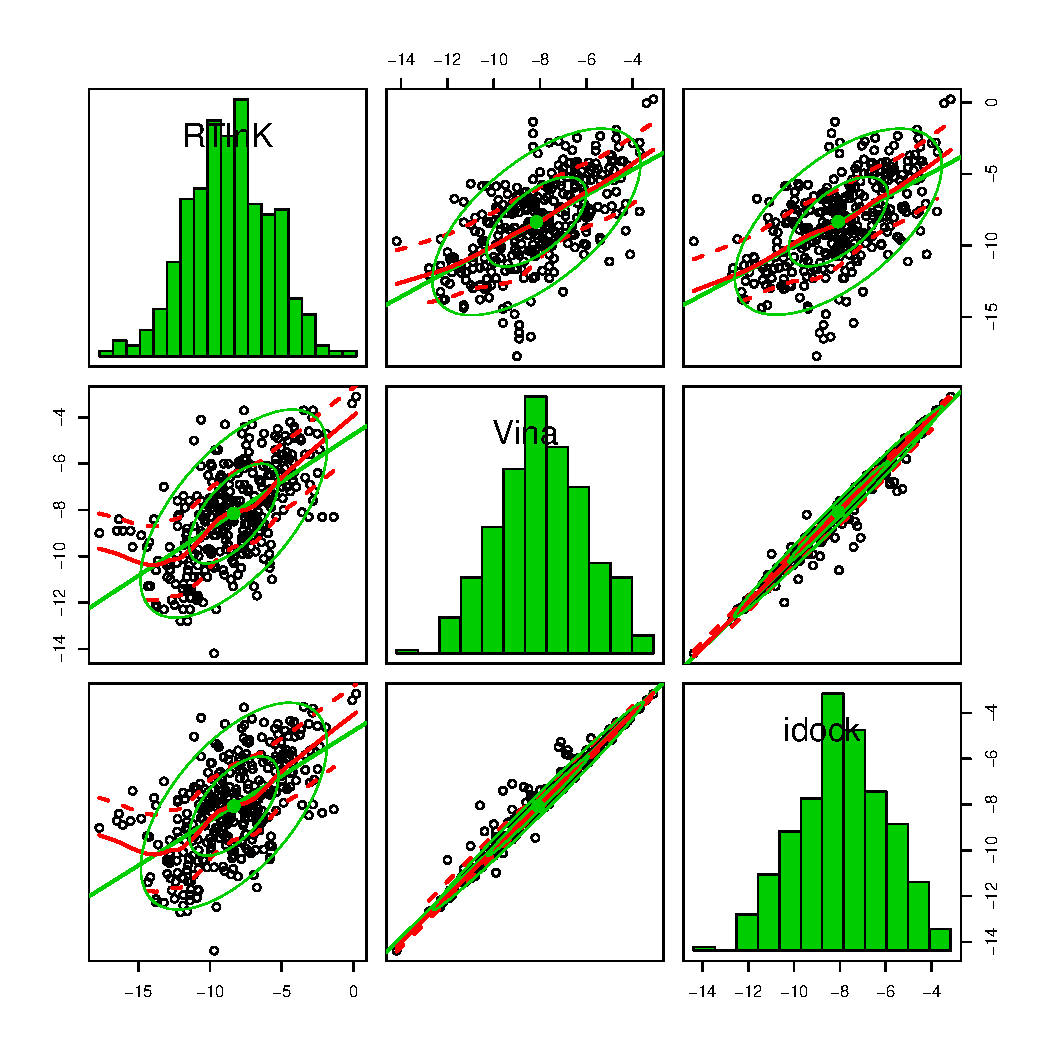
\includegraphics[width=0.485\linewidth]{idock/CSARFECorrelation.pdf}
}
\caption{Free energy correlation on PDBbind v2011 and CSAR NRC HiQ Set 24Sept2010.}
\label{idock:FECorrelation}
\end{figure*}

\subsection{Benchmark of Virtual Screening}

We collected 12 receptors from the PDB (Protein Data Bank) database \cite{540,537}, and 1000 ligands with a molecular weight of 200-300g/mol2, 1000 ligands with a molecular weight of 300-400g/mol2, and 1000 ligands with a molecular weight of 400-500g/mol2 from the clean subset of the ZINC database \cite{532,1178}. The 3000 ligands (Figure \ref{idock:MWT-NRB}) were docked against the 12 receptors by Vina and idock. Since Vina can dock only one ligand in each run, a bash script containing 1000 lines was executed instead, with each line being an execution of Vina to dock one individual ligand. The GNU Time utility was used as profiler.

\begin{figure*}
\centering
\subfloat
{
  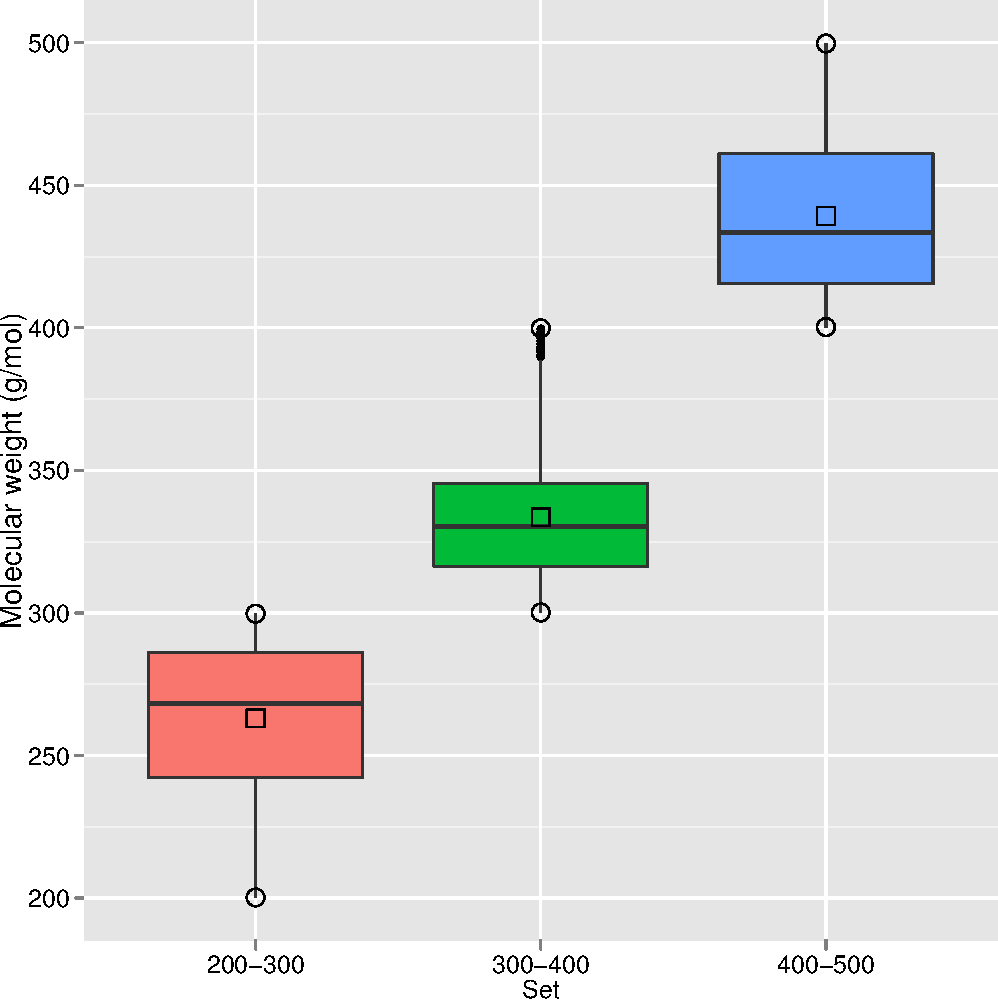
\includegraphics[width=0.485\linewidth]{idock/MWT.pdf}
}
\subfloat
{
  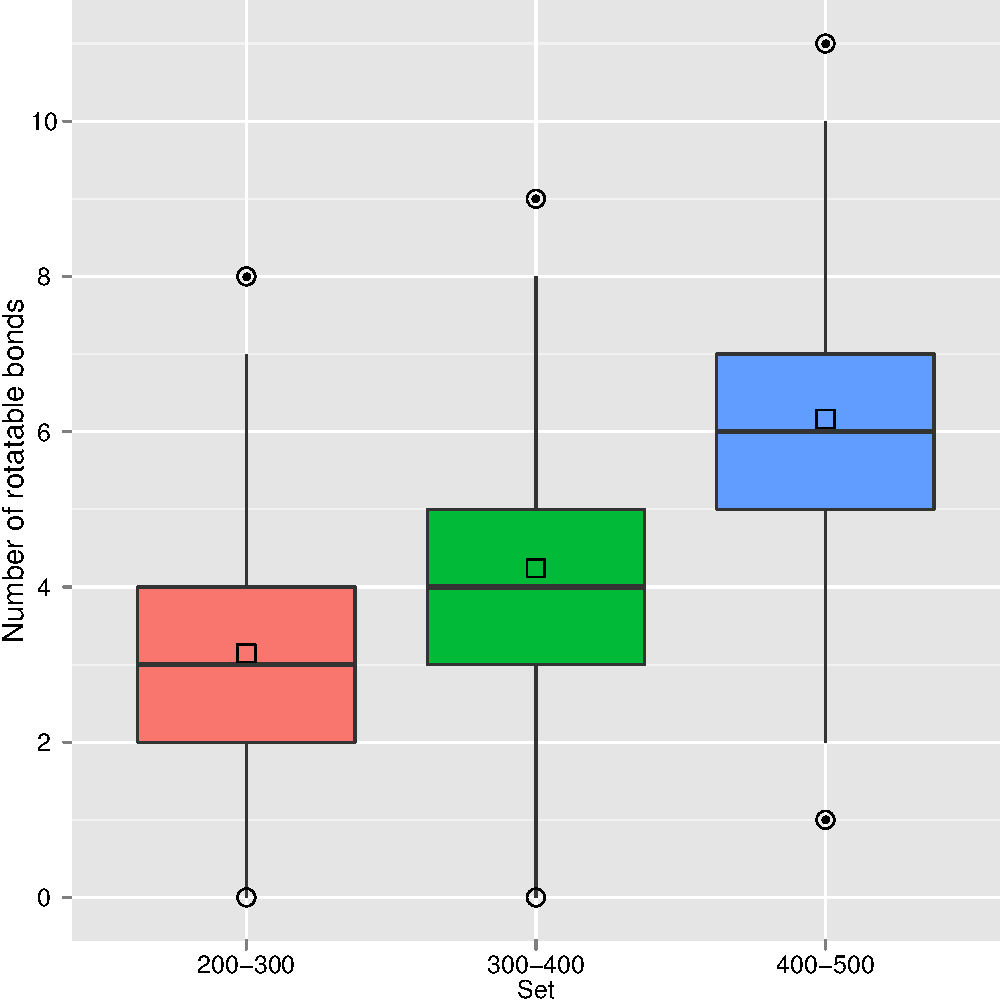
\includegraphics[width=0.485\linewidth]{idock/NRB.pdf}
}
\caption{Boxplot of molecular weight and number of rotatable bonds of ligands of the three molecular weight sets.}
\label{idock:MWT-NRB}
\end{figure*}

Table \ref{idock:ExecutionTime} compares the CPU time and elapsed time of both programs. The execution time varies a lot from receptor to receptor and from molecular weight set to set, so does the ratio. Conclusively idock outperforms Vina by at least 8.69 and at most 37.51 times.

\begin{table}
\centering
\begin{tabular*}
{\linewidth}
{@{\extracolsep{\fill}}crrrrrr}
\toprule
& \multicolumn{2}{c}{200-300g/mol} & \multicolumn{2}{c}{300-400g/mol} & \multicolumn{2}{c}{400-500g/mol}\\
& CPU & Elapsed & CPU & Elapsed & CPU & Elapsed\\
\midrule
\multicolumn{7}{l}{\textbf{1HCL} human cyclin-dependent kinase 2}\\
Vina  & 12.57 &  3.33 & 22.55 &  5.91 & 51.62 & 13.41\\
idock &  0.63 &  0.16 &  0.92 &  0.24 &  1.38 &  0.36\\
\multicolumn{7}{l}{\textbf{1J1B} human tau protein kinase I}\\
Vina  &  9.07 &  2.47 & 14.69 &  3.92 & 32.28 &  8.49\\
idock &  0.78 &  0.21 &  1.25 &  0.33 &  2.35 &  0.62\\
\multicolumn{7}{l}{\textbf{1LI4} human S-adenosylhomocysteine hydrolase}\\
Vina  & 11.82 &  3.30 & 19.08 &  5.22 & 39.41 & 10.64\\
idock &  0.89 &  0.23 &  1.55 &  0.40 &  3.15 &  0.82\\
\multicolumn{7}{l}{\textbf{1V9U} human rhinovirus 2 coat protein VP1}\\
Vina  &  9.80 &  2.95 & 15.55 &  4.62 & 29.75 &  8.49\\
idock &  0.97 &  0.25 &  1.64 &  0.42 &  3.42 &  0.89\\
\multicolumn{7}{l}{\textbf{2IQH} influenza A virus nucleoprotein NP}\\
Vina  &  9.51 &  2.66 & 15.03 &  4.08 & 29.64 &  7.83\\
idock &  0.92 &  0.24 &  1.59 &  0.41 &  3.41 &  0.88\\
\multicolumn{7}{l}{\textbf{2XSK} Escherichia coli curli protein CsgC - SeCys}\\
Vina  & 10.44 &  2.71 & 17.89 &  4.61 & 40.58 & 10.41\\
idock &  0.71 &  0.19 &  1.16 &  0.30 &  2.16 &  0.56\\
\multicolumn{7}{l}{\textbf{2ZD1} HIV-1 reverse transcriptase}\\
Vina  &  9.78 &  2.70 & 17.67 &  4.76 & 42.03 & 11.33\\
idock &  0.97 &  0.25 &  1.52 &  0.39 &  2.60 &  0.69\\
\multicolumn{7}{l}{\textbf{2ZNL} influenza virus RNA polymerase subunit PA}\\
Vina  &  9.49 &  2.60 & 15.04 &  4.01 & 29.97 &  7.82\\
idock &  0.89 &  0.23 &  1.56 &  0.40 &  3.41 &  0.87\\
\multicolumn{7}{l}{\textbf{3BGS} human purine nucleoside phosphorylase}\\
Vina  &  9.59 &  2.57 & 16.50 &  4.37 & 38.42 & 10.14\\
idock &  0.95 &  0.25 &  1.55 &  0.40 &  2.81 &  0.74\\
\multicolumn{7}{l}{\textbf{3H0W} human S-adenosylmethionine decarboxylase}\\
Vina  &  9.85 &  2.64 & 17.67 &  4.70 & 41.69 & 11.04\\
idock &  0.88 &  0.23 &  1.35 &  0.35 &  2.20 &  0.58\\
\multicolumn{7}{l}{\textbf{3IAR} human adenosine deaminase}\\
Vina  & 11.25 &  3.03 & 20.21 &  5.39 & 46.93 & 12.53\\
idock &  0.80 &  0.21 &  1.21 &  0.32 &  2.01 &  0.53\\
\multicolumn{7}{l}{\textbf{3KFN} HIV protease}\\
Vina  & 10.53 &  2.80 & 18.37 &  4.83 & 42.43 & 11.03\\
idock &  0.77 &  0.20 &  1.20 &  0.32 &  2.09 &  0.55\\
\multicolumn{7}{l}{\textbf{Average across the above 12 receptors}}\\
Vina  & 10.31 &  2.81 & 17.52 &  4.70 & 38.73 & 10.26\\
idock &  0.85 &  0.22 &  1.38 &  0.36 &  2.58 &  0.67\\
\bottomrule
\end{tabular*}
\caption{CPU time and elapsed time in hours of docking 3000 clean ligands of 3 molecular weight sets against 12 receptors by Vina and idock.}
\label{idock:ExecutionTime}
\end{table}

\section{Discussion and Conclusion}

We have developed idock for protein-ligand docking, inheriting from Vina the accurate scoring function and the efficient optimization algorithm, and meanwhile introducing a fruitful of innovations in C++ implementations, data structures, numerical models, and Monte Carlo algorithms. idock implements its own thread pool to maintain a high CPU utilization throughout the entire screening procedure. It intensively utilizes modern C++11 techniques, particularly Rvalue references to avoid frequent reallocations of array data. It flattens Vina's tree-like recursive data structures into simple array structures to guarantee a high data cache hit rate. It automatically detects and deactivates inactive torsions and thus reduces the dimension of variables to optimize.

In Vina's official forum, there are tremendous requests for the support for virtual screening. The development of idock perfectly complements Vina. idock has built-in support for virtual screening. It searches for ligands in a user-specified folder and docks them one by one. It reuses threads and grid maps across multiple ligands. idock has very similar input and output arguments as Vina, so it should be quite easy for existing Vina users to transit to idock. Vina supports flexible receptor docking by rotating flexible side-chains. However, at the moment we have not yet implemented flexible receptor docking, which has been proved helpful in some cases \citep{1084}, so users who need this kind of docking should refer to Vina.

We performed large-scale protein-ligand docking with idock, and noticed that the high-rank ligands were usually those comparatively rigid ligands with few active torsions. Such phenomenon can be explained by equation \eqref{eqn:FlexibilityPenalty}. Fewer active torsions imply smaller denominator, or larger value in other words. We are considering replacing free energy by some ligand efficiency indexes \citep{335,336,337} for ranking.

\section{Availability}

idock is free and open source under Apache License 2.0. Precompiled executables for 32-bit and 64-bit Linux, Windows, Mac OS X, FreeBSD and Solaris, 13 docking examples, and a doxygen file for generating API documentations are available at https://github.com/HongjianLi/idock. Grapical tutorials are available at http://idock.cse.cuhk.edu.hk.

\chapterend
